\chapterimage{tubes.jpg}

\chapter{Layer 4: Transport}\label{sec:layer4}

\begin{minipage}{0.4\linewidth}
\begin{center}
\begin{bytefield}{16}
\bitbox{16}{Layer 7: Application} \\
\bitbox{16}{\color{color1} Layer 4: Transport} \\
\bitbox{16}{Layer 3: Internet} \\
\bitbox{16}{Layer 2: Network (LAN)} \\
\bitbox{16}{Layer 1: Physical} \\
\end{bytefield}
\end{center}
\end{minipage}
\begin{minipage}{0.6\linewidth}
\begin{center}
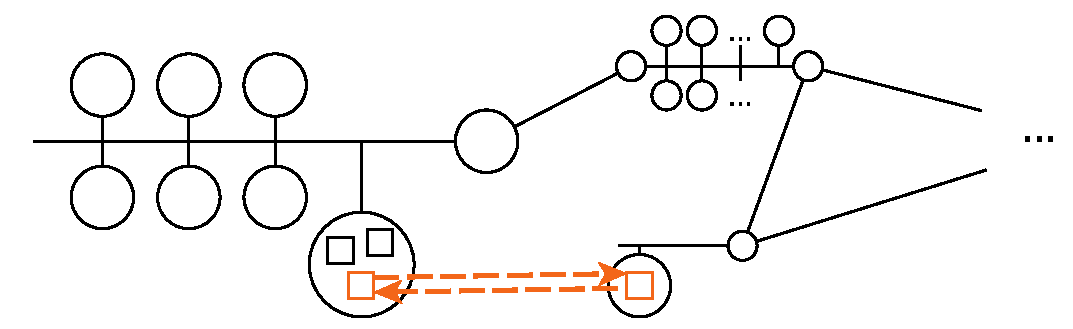
\includegraphics[width=\linewidth]{network_layer4.pdf}
\end{center}
\end{minipage}


% la ventana controla el flujo porque, si envio y recivo rápido, - envío el siguiente paquete antes, y sé que puedo porque la otra parte confirma al mismo ritmo.
